\documentclass[12pt]{article}
\usepackage[utf8]{inputenc}
\pagenumbering{arabic}
\usepackage{graphicx}
\usepackage{amstext}
\usepackage[usenames, dvipsnames]{color}
\usepackage{array}
\usepackage{float}
\graphicspath{ {images/} }


\begin{document}

\begin{titlepage}
    \begin{center}
    \begin{figure}
        \centering
        
\includegraphics[scale=0.2]{logoPolimi.png}
        \vspace{1.5cm}
    \end{figure}

    \Huge\textbf{Software Engineering 2 Project - Travlendar+}
    \rule{12cm}{0.5pt}
    \Huge\textbf{RASD - Requirement Analysis and Specification Document}
    \today
    \end{center}
    
    \vspace{3cm}
    
    \begin{flushleft}
        \LARGE\textbf{Authors: }
        \newline\newline
        \Large\texttt{}{Francisco Cristóvão \\ Samsom Beyene}
    \end{flushleft}



\end{titlepage}

\newpage
  \tableofcontents
\newpage

\section{Introduction}

\subsection{Purpose}

The main goal of this project is to create a calendar-based application which provides the user a flexible and fully-featured calendar support that considers the travel time between meetings. With this in mind, the application will:
\begin{itemize}
\item compute and account for travel time between appointments, and prevent conflicts between them
\item support the user in his/her travels, adding automatically the travel time to the calendar between meetings, and suggesting the best travel option based on the available time
\end{itemize}

\subsection{Scope}
Travlendar+ is a calendar-based application that provides the user a convenient way of organizing his/her daily schedule, maximizing its productiveness and minimizing the worthless time of his/her day. This application was not only thought for the regular businessman/businesswoman, who travel in between meetings the whole day and have no time to spare, but also for the parents with a more regular daily schedule, who just want to get the best of their time while being able to pick their kids from school and take them to other activities, always being on time.
Of course the system will fully support the features of a regular calendar application (booking of appointments in a specific time and location), but in a "smart" way, being able to detect and warn the user if a new appointment is not feasible because it has a conflict (the start of it doesn't allow the needed travel time after the end of the last appointment). The application is meant to be used in the City of Milan, and so it will take advantage of the wide range of travel means and services already existing in the city, from public transports to shared bikes and cars. With the information gathered from those services, it will be able to suggest the best travel mean for the user to move between appointments, based on the available travel time, total cost, current weather and even user preferences.


\subsection{Definitions, Acronyms, Abbreviations}
API: Application Programming Interface\\
RASD: Requirements Analysis and Specification Document\\
MTBF: Mean Time Between Failure
Home Screen: User interface screen that shows the current appointments.

\subsection{Revision History}

\subsection{Reference Documents}
Assignment document: Mandatory Project Assignments.pdf

\subsection{Document Structure}
Other than this introductory chapter, this RASD is organized in five more chapters. Chapter two is meant to provide an overview of the systems functionalities, the type of users it is meant for and the different kinds of interactions it contemplates, not only with the users themselves, but also with other systems. Some of the systems requirements are also slightly discussed in this chapter, even though they’ll be analysed in the following chapter. In the third chapter (as mentioned above) the systems requirements, attributes and constraints are analysed and discussed with the appropriate detail and depth, specifying exactly how they should be.
The fourth chapter deals with the formal analysis of the system using and Alloy model. It includes the Alloy model of the system, with a brief discussion on its purpose and on the relevance of using Alloy as a tool to validate our solution, given the problem we had to solve.
In the fifth chapter the effort spent by each of the group members is described by specifying the number of hours each member of the group worked on the development of this document.

\section{Overall Description}

\subsection{Product Perspective}
The application will need to communicate with both Public transport systems, bike or car sharing system of the city and Google maps API to find the exact status of available (active) types of transportation with their corresponding locations. These information’s helps the application to exactly locate the position of the user and meeting place so that it can assign the travel means with its calculated time. In addition, the application also retrieves the weather conditions while making some decisions. 
Since this application is data centric product it will need somewhere to store the schedules. For that a database is used. So the mobile application will communicate with the database (probably distributed database) to add, modify or view the schedule. All the database communication will go over the Internet.
    \begin{figure}[ht]
        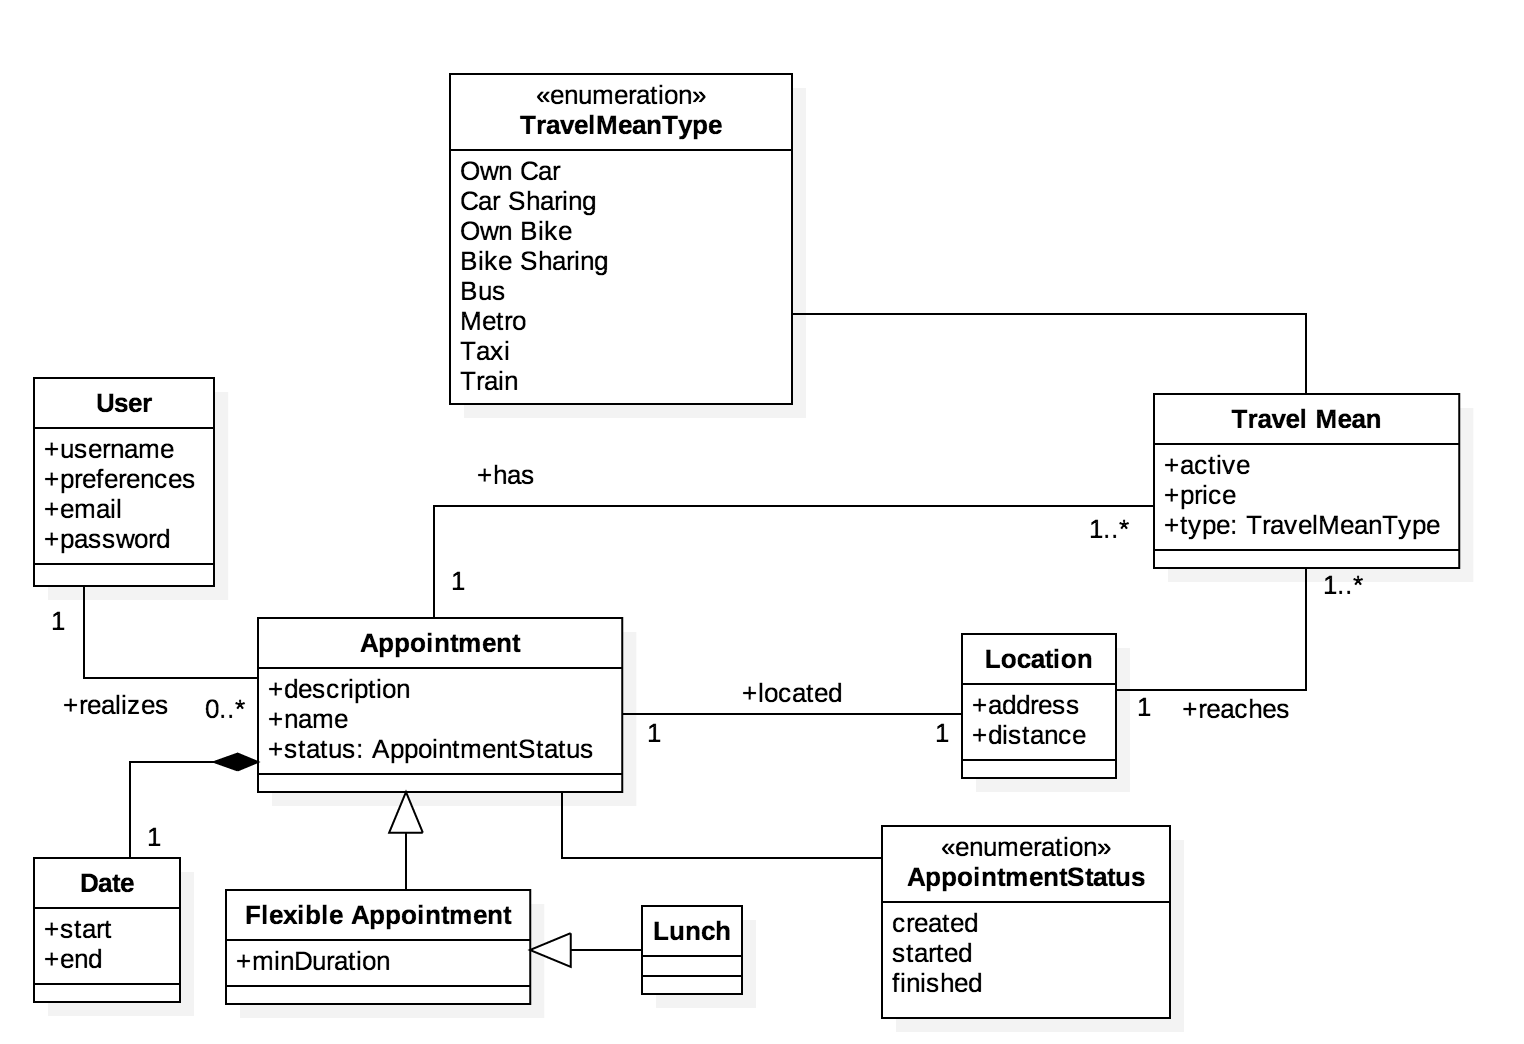
\includegraphics[scale=0.52]{domainModel.png}
        \caption{Class Diagram of the domain}
    \label{fig:domainModel}
    \end{figure}
    
\subsection{Product Functions}
The main functionalities supported by the system will be:
\begin{itemize}
    \item Allow the user to book an appointment with a given time, location and duration
    \item Suggest to the user the best travel means for him to use in between appointments, based on his preferences, the time available and the weather
\end{itemize}

\subsection{User Characteristics}
The system aims at satisfying the needs of many different types of users. The first type is the "businessman" user, the user that is always in a tight schedule and needs a tool like our system to simplify the way he books and turns up to the appointments. The second type is the opposite of the "businessman" user. It's a user that has a less busy life and only needs the system to remind him of the appointments without having to worry about how to get there or when to leave to arrive on time. There's also a third type of user which is placed in between the two described previously: also has a tight office schedule but still has time for personal activities, and needs the system to help him reach this balance in the most efficient way.
All of this types of users are of working age (20 to 70 years old, being this a small deviation of the official definition, which is from 15 to 64 years old)\footnote{Definition from OECD: https://data.oecd.org/pop/working-age-population.htm} and know how to use a smartphone.

\subsection{Assumptions, dependencies and constraints}
[D1] The username must be unique.\\{}
[D2] The system will have access to the phone GPS functionality.\\{}
[D3] The phone will always have a connection to the internet (WiFi or mobile data).\\{}
[D4] The users authorize the system to provide user data (when needed) to the third-party applications it interacts with.\\{}
[D5] The external services used by the system are assumed to be always reachable.\\{}


\section{Specific Requirements}

\subsection{External Interface Requirements}

\subsubsection{User Interfaces}
These Mockups represent a basic idea e of how the applications user interface will look like on the first release.

\subsubsection{Hardware Interfaces}
In the first release no Hardware Interfaces will be necessary, since the system doesn't need to interact physically with other systems.

\subsubsection{Software Interfaces}
Given the wide range of features the system offers, it will need to have several software interfaces. There has to be a way of storing all the user-related data (mainly login and preferences data). In that sense, the system will use a \textbf{MySQL API} to connect with a MySQL database server, where all the app data will be stored.\\
The system will also need different kinds of information about the users location and its surrounding, in order to compute the travel time between appointments. To support this functionality, the system will use \textbf{Google Maps Geolocation API} and \textbf{Google Maps API}. The first one will provide information about the user exact location and the second one will provide the real-time information about maps and traffic, and allow it to calculate the best route between two different appointments.\\
To have access to the current weather, the system will use \textbf{AccuWeather API}, which will provide information about the current weather either where the user is or where the user is going.
At last, the system also needs to get all sorts of information from many different travel means. In order to get this information, it will have a software interface with \textbf{ATM Milano} (public transport schedule and routes), \textbf{Drive Now API} (for the car sharing system) and \textbf{Ofo API} (for the bike sharing system).



\subsubsection{Communication Interfaces}
Communication interfaces ensure the communication between the system and the other software interfaces (third party service providers).
The communication between the system and those service providers is crucial because the system depends on those services in order to perform its functions. Given this, the systems communication interface must be either WiFi or mobile data, and the service providers communication interface can be of any type, as long as it ensures that they are connected to the internet. The protocol used shall be HTTPS, in order to keep the communications secure.

\subsection{Functional Requirements}

{[G1]} Allow a visitor to become a user after providing the required information and credentials.
\begin{itemize}
    \item{[R]} The system shall allow the visitor to begin the registration process when he accesses the system. 
    \item{[R]} The system shall ask the visitor for the required information and credentials during the registration process
    \item{[R]} The system shall register the visitor as a user when the registration process ends.
    \item {[D]} The username and email must be unique.
\end{itemize}
{[G2]} Allow a user to create an appointment.
\begin{itemize}
    \item{[R]} The system shall allow the user to login to the system when providing his valid login credentials.
    \item{[R]} The system shall allow the user to fill in all the needed information about the appointment.
    \item{[R]} The system shall create a warning if the appointments location is unreachable.
    \item{[R]} The system shall not allow the user to create an appointment if the location is unreachable.
    \item{[R]} The system shall allow the user to select if the scheduled hour for the appointment is flexible or not.
    \item{[R]} The system shall create the appointment if all the data inserted by the user is valid.
    \item {[D]} The location of the appointment will always be inserted correctly.
\end{itemize}
{[G3]} Allow a user to edit an appointment.
\begin{itemize}
    \item{[R]} The system shall allow the user to login to the system when providing his valid login credentials.
    \item{[R]} The system shall allow the user to edit all the provided information about the appointment.
    \item{[R]} The system shall create a warning if the appointments new location is unreachable.
    \item{[R]} The system shall not allow the user to submit the changes if the new location is unreachable.
    \item{[R]} The system shall submit the changes to the appointment if all the data inserted by the user is valid.
    \item{[R]} The system shall re-calculate the best travel mean to get to the appointments directly before the one deleted.
    \item{[R]} The system shall re-calculate the best travel mean to get to the appointments directly after the one deleted.
    \item {[D]} The location of the appointment will always be inserted correctly.
\end{itemize}
{[G4]} Allow a user to delete an appointment.
\begin{itemize}
    \item{[R]} The system shall allow the user to login to the system when providing his valid login credentials.
    \item{[R]} The system shall allow the user delete the appointment and all the information referring to it.
    \item{[R]} The system shall re-calculate the best travel mean to get to the appointments directly before the one deleted.
    \item{[R]} The system shall re-calculate the best travel mean to get to the appointments directly after the one deleted.
\end{itemize}
{[G5]} Allow a user to know which is the best travel mean to get to an appointment.
\begin{itemize}
    \item{[R]} The system shall allow the user to login to the system when providing his valid login credentials.
    \item{[R]} The system shall compute the best route for the user to take to an appointment.
    \item{[R]} The system shall compute the best travel mean for the user, taking into account the computed route to an appointment.
    \item{[R]} The system shall display the best travel mean for each appointment the user has created.
    \item{[D]} The best route to get to an appointment will always be computed correctly.
    \item{[D]} The best travel mean to get to an appointment will always be computed correctly.
    
\end{itemize}
{[G6]} Allow a user to define preferences related to travel means.
\begin{itemize}
    \item{[R]} The system shall allow the user to login to the system when providing his valid login credentials.
    \item{[R]} The system shall allow the user to enable all the travel means he wants the system to consider when computing the best way to move in between appointments.
    \item{[R]} The system shall allow the user to disable all the travel means he doesn't want the system to consider when computing the best way to move in between appointments.
\end{itemize}
{[G7]} Allow a user to define constraints related to travel means.
\begin{itemize}
    \item{[R]} The system shall allow the user to login to the system when providing his valid login credentials.
    \item{[R]} The system shall allow the user to select the distance he is willing to walk from one appointment to another.
    \item{[R]} The system shall allow the user to select an hour of the day from when public transportation shall not be used.
    \item{[R]} The system shall allow the user to select a combination of public transportation in order to minimize his carbon footprint.
\end{itemize}


\subsubsection{Use Case Description}
\paragraph{Visitor Registration}

\begin{center}
    \begin{tabular} { |p{0.25\textwidth}|p{0.7\textwidth}| }
        \hline
        \textbf{Actors} & Visitor \\ 
        \hline
        \textbf{Goals} & {[G1]} \\ 
        \hline  
        \textbf{Preconditions} & There are no preconditions. \\ 
        \hline
        \textbf{Events Flow} & \begin{enumerate} 
                            \setlength{\itemsep}{0.5pt}
                            \item The Visitor opens Travlendar application.
                            \item The Visitor clicks on the "Sign up" button to start the registration process. 
                            \item The Visitor fills all the mandatory fields with his data. 
                            \item The Visitor clicks on the "Register Button".
                            \item The system saves the data.
                            \end{enumerate} \\
        \hline
        \textbf{Postconditions} & The Visitor ends the registration process successfully and from now on is a user of the system. \\
        \hline
        \textbf{Exceptions} & \begin{enumerate} 
                            \setlength{\itemsep}{0.5pt}
                            \item The Visitor is already a user. 
                            \item The Visitor doesn't fill all the mandatory fields or fills them with invalid data.
                            \item The Visitor chooses a username which is already associated with another user.
                            \item The Visitor chooses an email which is already in use by another user. 
                            \end{enumerate} 
                            All exceptions are handled notifying the Visitor about the issue and going back to event 2 of the Event Flow described above.\\ 
        \hline
    \end{tabular}
\end{center}

\paragraph{User Login}
\begin{center}
    \begin{tabular} { |p{0.25\textwidth}|p{0.7\textwidth}| }
        \hline
        \textbf{Actors} & User \\ 
        \hline
        \textbf{Goals} & All goals except {[G1]} \\ 
        \hline  
        \textbf{Preconditions} & There are no preconditions. \\ 
        \hline
        \textbf{Events Flow} & \begin{enumerate} 
                            \setlength{\itemsep}{0.5pt}
                            \item The User opens Travlendar application.
                            \item The User inserts his username and password on the respective fields.
                            \item The User clicks on the "Log In" button.
                            \item The system redirects the user to the Home Screen screen.
                            \end{enumerate} \\
        \hline
        \textbf{Postconditions} & The User is successfully logged in to the system and redirected to the Home Screen. \\
        \hline
        \textbf{Exceptions} & \begin{enumerate} 
                            \setlength{\itemsep}{0.5pt}
                            \item The User inserts an invalid username or email.
                            \end{enumerate} 
                            All exceptions are handled notifying the User about the issue and going back to event 2 of the Event Flow described above.\\ 
        \hline
    \end{tabular}
\end{center}


\paragraph{User creates an appointment}

\begin{center}
    \begin{tabular} { |p{0.25\textwidth}|p{0.7\textwidth}| }
        \hline
        \textbf{Actors} & User \\ 
        \hline
        \textbf{Goals} & {[G2]} \\ 
        \hline  
        \textbf{Preconditions} & The User must be already logged in. \\ 
        \hline
        \textbf{Events Flow} & \begin{enumerate} 
                            \setlength{\itemsep}{0.5pt}
                            \item The user clicks on the "New Appointment" button
                            \item The system shows a form with the required data fields in order for the appointment to be created.
                            \item The User fills the form.
                            \item The User clicks on the "Create Appointment" button.
                            \item The system redirects the user to the Home Screen.
                            \end{enumerate} \\
        \hline
        \textbf{Postconditions} & The User successfully creates an appointment and is redirected to the Home Screen. \\
        \hline
        \textbf{Exceptions} & \begin{enumerate} 
                            \setlength{\itemsep}{0.5pt}
                            \item The User creates an appointment which is unreachable.
                            \end{enumerate} 
                            The exception is handled notifying the User about the issue and going back to event 1 of the Event Flow described above.\\ 
        \hline
    \end{tabular}
\end{center}

\paragraph{User deletes an appointment}

\begin{center}
    \begin{tabular} { |p{0.25\textwidth}|p{0.7\textwidth}| }
        \hline
        \textbf{Actors} & User \\ 
        \hline
        \textbf{Goals} & {[G4]} \\ 
        \hline  
        \textbf{Preconditions} & The User must have created at least one appointment. \\ 
        \hline
        \textbf{Events Flow} & \begin{enumerate} 
                            \setlength{\itemsep}{0.5pt}
                            \item The user press clicks on the appointment he wants to delete.
                            \item The system shows a "Delete" button.
                            \item The User clicks on the "Delete" button.
                            \end{enumerate} \\
        \hline
        \textbf{Postconditions} & The User successfully deletes an appointment and stays on the Home Screen. \\
        \hline
        \textbf{Exceptions} & There are no exceptions.\\ 
        \hline
    \end{tabular}
\end{center}

\paragraph{User looks for the best travel mean to get to an appointment}
\begin{center}
    \begin{tabular} { |p{0.25\textwidth}|p{0.7\textwidth}| }
        \hline
        \textbf{Actors} & User \\ 
        \hline
        \textbf{Goals} & {[G5]} \\ 
        \hline  
        \textbf{Preconditions} & The User must have created at least one appointment. \\ 
        \hline
        \textbf{Events Flow} & \begin{enumerate} 
                            \setlength{\itemsep}{0.5pt}
                            \item The looks for the appointment he wants on the Home Screen and reads the data about it
                            \end{enumerate} \\
        \hline
        \textbf{Postconditions} & The User successfully deactivated Bike Sharing as a mean of transportation and is redirected to the Home Screen. \\
        \hline
        \textbf{Exceptions} & There are no exceptions.\\ 
        \hline
     \end{tabular}
\end{center}

\paragraph{User deactivates Bike Sharing as a travel mean}
\begin{center}
    \begin{tabular} { |p{0.25\textwidth}|p{0.7\textwidth}| }
        \hline
        \textbf{Actors} & User \\ 
        \hline
        \textbf{Goals} & {[G6]} \\ 
        \hline  
        \textbf{Preconditions} & The User must be already logged in. \\ 
        \hline
        \textbf{Events Flow} & \begin{enumerate} 
                            \setlength{\itemsep}{0.5pt}
                            \item The user clicks on the "Settings" button
                            \item The system shows a slide button form, one for each mean of transportation.
                            \item The User sets the Bike Sharing slide button to deactivated.
                            \item The User clicks on the "Done" button.
                            \end{enumerate} \\
        \hline
        \textbf{Postconditions} & The User successfully deactivated Bike Sharing as a mean of transportation and is redirected to the Home Screen. \\
        \hline
        \textbf{Exceptions} & There are no exceptions.\\ 
        \hline
     \end{tabular}
\end{center}





\subsection{Performance Requirements}
The system has to be able to respond to a possibly large number of requests (depending on the amount of users the system will have). Taking into account other (less powerful but widely used) calendar and transport applications, an infrastructure that supports a maximum workload on the order of hundreds of thousands of requests shall be enough to satisfy all the possible simultaneous requests after the release. The infrastructure must have a good Scalability in order to increase the maximum workload in case the user base increases too. The response times of the system shall be\footnote{According to Jakon Nielsen book on Usability}:
\begin{itemize}
    \item 0.1 second for the tasks that require almost no computing power (changing menus in the systems case), in order for the user to feel that the system is reacting instantaneously
    \item 1 second for the tasks that require a normal amount of computing power, in order for the users flow of thought to stay uninterrupted (deleting an appointment in the systems case)
    \item 10 second for the task that require significant computing power, in order for the user’s flow of thought to stay uninterrupted (computing the best travel route and consequent travel mean to get to an appointment in the systems case). The users must also receive some sort of feedback during the wait, so they can know what to expect.
\end{itemize}
A user is assumed to have a stable internet connection in order to achieve these response times.


\subsection{Design Constraints}
\subsubsection{Standard Compliance}
The system must require the users permission to provide their location, preferences and schedule to the external services it uses (transport services and weather services), in order to manage sensible data always respecting the privacy law.

\subsubsection{Hardware Limitations}
The user will need a mobile phone with GPS and Wi-fi/Mobile Data always on when using the app, other than the obvious space for the application package.

\subsubsection{Any other Constraint}

\subsection{Software System Attributes}

\subsubsection{Reliability}
When deployed, no bugs must be detected on the system, and the system must be fully available and functional for 99,9\% of the calendar year. 

\subsubsection{Availability}
The services that the system provides must be available 24/7. Obviously, taking into account that this requirement is really hard to fulfill, very small deviations from this requirement will be considered acceptable.

\subsubsection{Security}
Users credentials and payment information are critical data that will be stored in the systems database. Since the system communicates with external systems, the security and inaccessibility (when not needed) of this data is a big concern that has to be assured. All of the data related to the appointments has to be secured too since it can be sensible information. 

\subsubsection{Maintainability}
To measure the systems maintainability a metric shall be used. This metric needs to be tracked during the development and kept as low as possible, in order to avoid high maintainability costs subsequently. It's obvious that the system must have a high maintainability, which means that the probability of performing a successful repair action within a given (necessary) time must be high (higher than 95\%).

\subsubsection{Portability}
The first release of the system will be available for the mobile platform our target users use the most, IOS. Nonetheless, an Android version shall be released soom, and even a new platform may arise. So it's crucial that the system is built in a way which makes it easy to deploy in different platforms. The portability measure consists on the cost that deploying the system in a new platform implies, and in this case, this cost should be smaller than the cost of deploying other similar apps.

\section{Formal Analysis Using Alloy}

\section{Effort Spent}
\subsection{Francisco Cristóvão}

\begin{center}
\begin{tabular}{ |p{0.25\textwidth}|p{0.4\textwidth}|p{0.25\textwidth}| } 
 \hline
 \textbf{DATE} & \textbf{TASK} & \textbf{HOURS} \\ 
  \hline
 03/10/2017 & Requirements Analysis & 1 \\ 
  \hline
 08/10/2017 & Domain Model and Class Diagram & 1,5 \\ 
  \hline
  09/10/2017 & Purpose and Document Structure & 1 \\ 
  \hline
  11/10/2017 & Scope and Purpose & 1 \\ 
  \hline
  12/10/2017 & User, Software and Hardware Interfaces, Product Functions and User Characteristics & 4,5 \\ 
  \hline
  13/10/2017 & Software System Attributes & 3 \\ 
  \hline
  16/10/2017 & Goals and Requirements, Use case Description & 2 \\ 
  \hline
  17/10/2017 & Use Case Description and User Interface & 4 \\ 
  \hline
  18/10/2017 & Goals, Requirements and Domain Assumptions & 2 \\ 
  \hline
  \textbf{TOTAL} & \multicolumn{2}{c|}{20} \\ 
  \hline
\end{tabular}
\end{center}

\section{References}
https://belitsoft.com/php-development-services/software-requirements-specification-document-example-international-standard\\
https://en.wikipedia.org/wiki/Portability_testing\\
https://en.wikipedia.org/wiki/Maintainability\\
https://en.wikipedia.org/wiki/Software_reliability_testing
Jakon Nielsen book on Usability - response intervals data 

\end{document}